\chapter{Case Study}
All information about formatting a dissertation can be found on the library website at www.stevens.edu/library/services/phd.html.  Formatting information gets updated occasionally, so it is always good to check the requirements before submitting your dissertation.  

It is not required, but is strongly suggested that you make an appointment at the library to have the format of your dissertation reviewed before the final submission.  Dissertations can be rejected if they do not adhear to the formatting requirements.   

All information about formatting a dissertation can be found on the library website at www.stevens.edu/library/services/phd.html.  Formatting information gets updated occasionally, so it is always good to check the requirements before submitting your dissertation.  
It is not required, but is strongly suggested that you make an appointment at the library to have the format of your dissertation reviewed before the final submission.  Dissertations can be rejected if they do not adhear to the formatting requirements.   
All information about formatting a dissertation can be found on the library website at www.stevens.edu/library/services/phd.html.  Formatting information gets updated occasionally, so it is always good to check the requirements before submitting your dissertation.  

\begin{table}[htp]

\begin{center}
\begin{tabular}{|l|c|p{3.0in}|}
\hline
\multicolumn{3}{|c|}{Theoretical Dissertation Timeline}\\ \hline
Taskt&Time to Finish&Notes\\ \hline
Problem statement&10 hours&Initially very upbeat.\\ \hline
Research&3 days&Literature search to very previous studies.\\ \hline
Reformulation&4 hours&Presented and accepted by advisor\\ \hline
Research&20 days&Literature search to very previous  studies.\\ \hline
Experiments&14 days&Do some experiments and get results.\\ \hline
Format&1 day&Understand format guidelines for paper.\\ \hline
Write&years&Write the paper.\\ \hline
Revise&not too long&Proof read, etc.\\ \hline
Format&1-3 days&Verify correct report format is used.\\ \hline
See Library&1 hour&Meet with Doris to verify formatting.\\ \hline
Defend&1 day&Defend your research.\\ \hline
Revise&0 hours&It was perfect the first time.\\ \hline
Submit&1 day&Submit final dissertation to the library.\\ \hline
\end{tabular}
\end{center} 

\caption{Table of Tasks}\label{fig:erptsqfit}
\end{table}
It is not required, but is strongly suggested that you make an appointment at the library to have the format of your dissertation reviewed before the final submission.  Dissertations can be rejected if they do not adhear to the formatting requirements.   
All information about formatting a dissertation can be found on the library website at www.stevens.edu/library/services/phd.html.  Formatting information gets updated occasionally, so it is always good to check the requirements before submitting your dissertation.  
It is not required, but is strongly suggested that you make an appointment at the library to have the format of your dissertation reviewed before the final submission.  Dissertations can be rejected if they do not adhear to the formatting requirements.   
All information about formatting a dissertation can be found on the library website at www.stevens.edu/library/services/phd.html.  Formatting information gets updated occasionally, so it is always good to check the requirements before submitting your dissertation.  

It is not required, but is strongly suggested that you make an appointment at the library to have the format of your dissertation reviewed before the final submission.  Dissertations can be rejected if they do not adhear to the formatting requirements.   

\section{Further Analysis}  

\subsection*\normalsize\emph{Paper}
The original copy of the dissertation must be produced on good quality 8 1/2$''$ x 11$''$, 20 pound acid-free white paper. The paper should not be stapled, punched, bound, colored or printed on letterhead.

The two additional copies of the dissertation can be photocopied or produced on copier or laser paper.

\subsection*\normalsize\emph{Ink}
Black ink only is used to print your report.  If a graph or photograph contains color, that is fine. 

Latex is used to help in the printing of formulas.   The following formula would be difficult to reproduce in Microsoft Word: 
 \[
        \frac{d}{dx}\left( \int_{0}^{x} f(u)\,du\right)=f(x).
     \]

This Report was produced by LaTeX\footnote {\LaTeX\ is a fun typesetting program.} written by Barbara Arnett.  Barbara is not an expert with LaTeX, and anyone using LaTeX does not need to use this template.  It is simply provided to help with formatting, specifically with page numbers and images.  


%this subsection heading below will not show up in the table of contents.
\subsection*\normalsize\emph{Graphics} 

Graph paper may be used for original drawings, charts or illustrations. Original drawings may be in color or black and white, however, color is allowed for illustrations only; all text must appear in black. The original thesis must contain the original graphic or illustration, not a photocopy of the drawing, graphic or illustration.

If formulas and diagrams contain subscript and superscript characters, ensure they are large enough to read when printed in the final paper. 

\begin{figure}[htp]
\centering
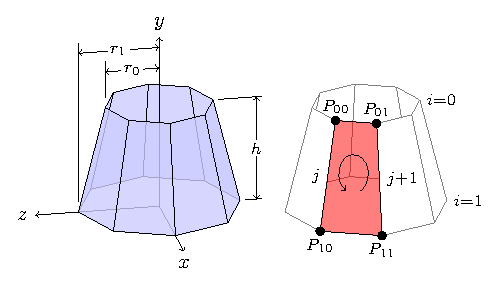
\includegraphics{casestudy/figures/3d-cone.pdf}
\caption{3D Cone}\label{fig:3d-cone}
\end{figure}

Photographs
Glossy prints of good reproducible quality, either black or white or color may be used. Photographs can be printed on 8 1/2$''$ x 11$''$ glossy finish paper, however, margin and page number requirements as stated above still apply for pages containing photographs. When attaching photographs to paper, double-sided tape may be used which causes the least amount of damage to the original paper. 

Graphics that are oriented in a landscape position must be done in a manner that retains the page numbering in the upper right hand corner, as shown in figure 3.2.  This can be difficult in Microsoft Word, but it is possible.  To do this in Microsoft Word, create a new section, change the page to landscape, and place the page number in a text box.  The text box then is rotated on the landscape page.    Then begin a new section and resume portrait orientation.

\begin{sidewaysfigure}
\centering
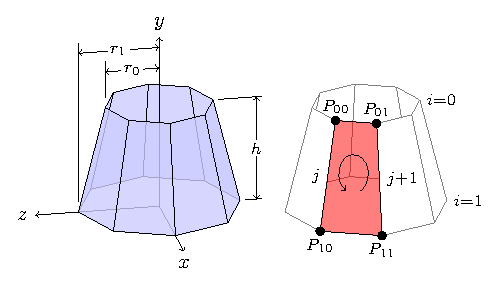
\includegraphics[height=5.0in, width=7.5in]{casestudy/figures/3d-cone.pdf}
\caption{This is an example of a landscape image within a page.  Note that the page number remains in the upper right hand corner of the page when the page is in the portrait position.}
\end{sidewaysfigure}